\documentclass{article}


\usepackage[utf8]{inputenc} % Поддержка UTF-8
\usepackage[russian]{babel} % Поддержка русского языка
\usepackage{amsmath, amsfonts, amssymb} % Для математических выражений и символов
\usepackage{geometry} % Настройка полей страницы
\geometry{top=2cm, bottom=2cm, left=2.5cm, right=2.5cm}
\usepackage{enumitem} % Списки с кастомными настройками
\usepackage{hyperref} % Для гиперссылок
\usepackage{graphicx}

\title{Теория функции комплексной переменной}
\author{Шарабарин Михаил}
\date{18.02.2025}

\begin{document}
\section{Интегрирование функции комлексного переменного}
$ \sqsupset \left[a,b\right]  $ отрезок вещественной прямой. Непрерываное 
отображение из вещественной части  отрезка $\left[a,b\right]$ в комплексную пл-ть
называется непрерывной кривой 

\begin{figure}[h]
    \centering
    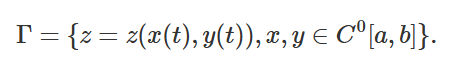
\includegraphics[width=0.5\textwidth]{2025-02-18-14-46-39.png}
    \caption{Описание изображения}
    \label{fig:example}
\end{figure}

\(C^0\) обозначает то что кривая непрерывная (но совсем не значит что диф-ма)
В записи \( C^0[a, b] \) число \textbf{0} указывает на \textbf{степень гладкости} функций, входящих в это пространство.

\section*{Что означает \( C^0[a, b] \)?}
\begin{itemize}
    \item \( C^0[a, b] \) — это множество \textbf{непрерывных функций} на отрезке \( [a, b] \).
    \item Число \textbf{0} означает, что функции \textbf{непрерывны}, но не обязательно дифференцируемы.
\end{itemize}

\section*{Аналогичные обозначения:}
\begin{itemize}
    \item \( C^1[a, b] \) — множество функций, которые \textbf{непрерывны} и имеют \textbf{непрерывную первую производную}.
    \item \( C^2[a, b] \) — функции, имеющие \textbf{непрерывную первую и вторую производные}.
    \item \( C^k[a, b] \) — функции, имеющие \textbf{непрерывные производные до порядка \( k \)}.
    \item \( C^\infty[a, b] \) — бесконечно \textbf{гладкие функции} (имеют все производные).
    \item \( C^\omega[a, b] \) — \textbf{аналитические функции}, которые можно разложить в ряд Тейлора.
\end{itemize}

Таким образом, в данном случае \textbf{\( C^0[a, b] \) говорит о том, что \( x(t) \) и \( y(t) \) — просто непрерывные функции, но могут не иметь производных}.


Кривая $\Gamma $ называется \textbf{кривой Жордана} если указанные отображения 
взаимно однозначны, за исключенем одной точки в которую могут отображаться кон-
цы отрезка (в таком случае замкнутая кривая). Это кривая без самопересечений.

Кривая Жордана называется \textbf{гладкой} если в каждой ее точке существует касательная
(отображение 
z
(
t
)
 - непрерывно дифференцируемо, то есть 
x
,
y
∈
C
1
[
a
,
b
]
, причем 
z
′
(
t
)
≠
0
).

кривая жордана называется спрямляемой, если она имеет длину. 

\end{document}